%-----------------------------------------------
% Template para criação de resumos de projectos/dissertação
% jlopes AT fe.up.pt,   Fri Jul  3 11:08:59 2009
%-----------------------------------------------

\documentclass[9pt,a4paper]{extarticle}

%% English version: comment first, uncomment second
%\usepackage[portuguese]{babel}  % Portuguese
\usepackage[english]{babel}     % English
\usepackage{graphicx}           % images .png or .pdf w/ pdflatex OR .eps w/ latex
\usepackage{times}              % use Times type-1 fonts
\usepackage[utf8]{inputenc}     % 8 bits using UTF-8
\usepackage{url}                % URLs
\usepackage{multicol}           % twocolumn, etc
\usepackage{float}              % improve figures & tables floating
\usepackage[tableposition=top]{caption} % captions
%% English version: comment first (maybe)
\usepackage{indentfirst}        % portuguese standard for paragraphs
%\usepackage{subfig}
\usepackage{todonotes}
%\usepackage{parskip}

%% page layout
\usepackage[a4paper,margin=30mm,noheadfoot]{geometry}

%% space between columns
\columnsep 12mm

%% headers & footers
\pagestyle{empty}

%% figure & table caption
\captionsetup{figurename=Fig.,tablename=Tab.,labelsep=endash,font=bf,skip=.5\baselineskip}

%% heading
\makeatletter
\renewcommand*{\@seccntformat}[1]{%
  \csname the#1\endcsname.\quad
}
\makeatother

%% avoid widows and orphans
\clubpenalty=300
\widowpenalty=300

\begin{document}

\title{\vspace*{-8mm}\textbf{\textsc{End-User Programming in Mobile Devices
through Re-usable Visual Components Composition}}
\author{\emph{Tiago Manuel da Silva Almeida}\\[2mm]
\small{Dissertation supervised by \emph{Prof.\ Hugo Sereno Ferreira}}\\
\small{and co-supervised by Tiago Boldt Sousa}}}
\date{}
\maketitle
%no page number 
\thispagestyle{empty}

\vspace*{-4mm}\noindent\rule{\textwidth}{0.4pt}\vspace*{4mm}

\begin{multicols}{2}

\section{Motivation}\label{sec:motiva}

The era where smartphones sales surpassed PCs has begun. In such era, end-users (the ones that ultimately use the smartphone) 
are demanding quantity and highly customizable applications in their devices. 
This makes it impractical for a software developers to ``foresee'' every possible development combination and provide all users with the best possible application for him. 

A possible solution to make customizable applications is to empower end-users with \emph{end-user programming} (EUP) tools. 
EUP is \emph{``the practice by which end users write computer programs to satisfy a specific need, but programming is not their primary job function''} \cite{EUSEReport}.
That EUP tool could be a collaborative framework, where novices and experts can co-exist and share their implementations, while end-users explore their requirements. With such scenario, expert programmers can create components that end-users can connect using a \emph{visual programming language} (VPL). Such tool could not only reduce the number of ``small'', similar, specific-tailored applications, but also foster discovery and experimentation by end-users.

\section{Objectives}\label{sec:goals}

While developing an EUP tool, we set our goals in answering to the following problems with a working prototype:

\begin{itemize}
	\item{\textbf{Smartphone's limitations in the implementation of a EUP solution} \\
    VPLs can be hard to use in small screens. How can we use visual elements without overflowing the screen? Is a typical data-flow solution with zoom enough? Can we use VPLs in small screens and work with solutions with medium to large number of components?}
	
	\item{\textbf{Defining an abstraction level for a collaborative framework} \\
	Higher abstraction levels may be good for end-users but they can limit the blocks produced by expert programmers. Can we achieve a balanced abstraction level for both end-users and expert programmers?}
  
	\item{\textbf{Block reuse in EUP} \\
    How can we approach reuse of components and incite end-users to use it?
    Could we benefit from a market for sharing components? What other reuse possibilities can be explored?}
	
\end{itemize}

\section{From Android to Scala: Steps into a EUP solution}\label{sec:work}

For approaching the problems at hand, we started by looking into literature regarding EUP problems \cite{Barriers2004} which quickly raised awareness on another topic: \emph{End-User Software Engineering} (EUSE).
Additionally, we found out that VPLs are a way to solve some of those problems \cite{Navarro2001}, so we also studied these languages.

With the gathered knowledge, a prototype for Android using concepts from VPLs was developed and improved according to end-users feedback obtained from informal experimentation. 
A common problem detected by end-users was the amount of blocks necessary to do simple tasks. To solve this issue we thought in a rewrite rule system and we decided to experiment a new language to do this system: Scala \cite{ProgrammingScala}.

\subsection{A Typed Block-based Prototype}

\todo{review and capitalize titles}

\begin{figure}[H]
\centerline{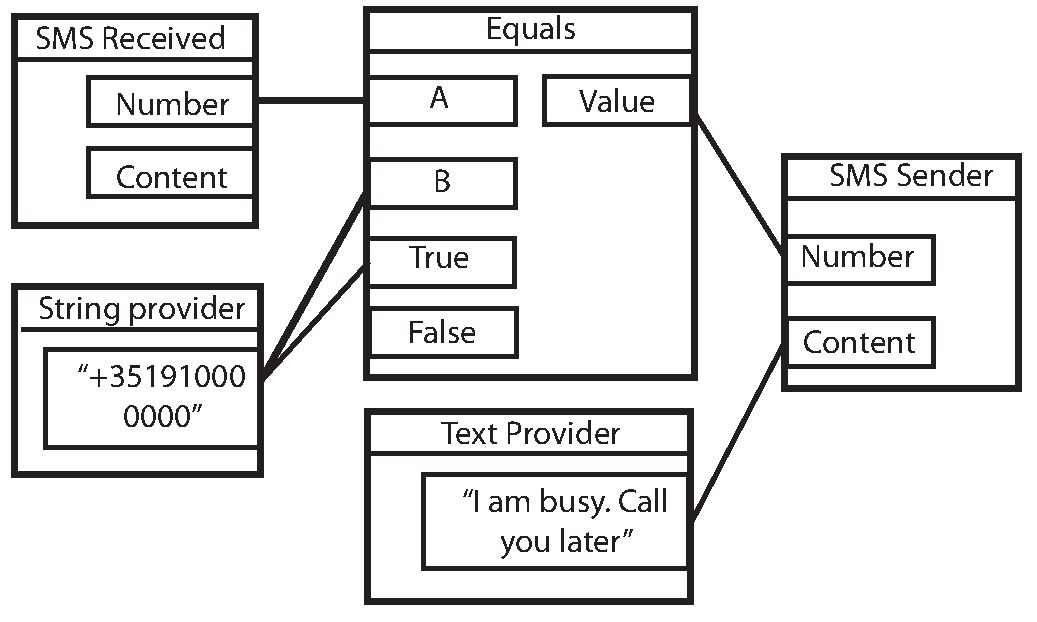
\includegraphics[scale=.43]{block_example.pdf}}
\label{fig:block}
\caption{A task composed by a set of blocks.} 
\end{figure}

Representing a function or an algorithm as a block, with inputs and outputs, was already used in software engineering, p.e., in black box testing \cite{BlackBoxTesting}. This metaphor was also thought for EUP, as described by Zin \cite{Zin2011}, where he states that a block is composed by a set of inputs and it returns data into outputs that can. in turn, be connected with other inputs.
Both outputs and inputs are called connectors and each connector has a type. A set of connected blocks is a block by itself that might be reused. 

A block can be shown to the end-user using a box with inputs on the left and outputs on the right.
Figure \ref{fig:block} shows that a block can connect its outputs with inputs from other block. This figure shows a task that automatically replies a message with the content ``I am busy. Call you later'' when a message is received from the number ``+351910000000''. The equal blocks has two set of inputs: \texttt{A} and  \texttt{B}, that are the values to be compared; \texttt{True} and  \texttt{False}, that are the values that will be used in case the expression \texttt{A == B} is true or false. The \texttt{Value} output will hold the value from \texttt{True} or \texttt{False} depending on the expression's result. 

Blocks can be developed by expert programmers and end-users can connect them. A set of connected blocks define a task, and a task is, itself, a block that can be connected with other blocks to create new tasks.

Tasks can be created in our prototype through an expansible two column layout. Initially there are two columns on the screen that can be used to add and connects blocks. When the end-users want to connect blocks to the blocks on the right column he can do a swipe gesture from the right to the left and the blocks from the right column will pass to the left column and a new empty column on the right appears.

\subsection{Experiments with a Rewrite Rule System}

Despite usability improvements introduced in the prototype based on end-users' feedback, we still needed a way to do automatic simplifications in a set of blocks, and other way to convert connectors' types without recurring
to extra blocks. We tried to use Scala for solving these problems.

Scala provide two main features that were relevant for the described problems: pattern matching and implicit conversions. Pattern matching allowed us to search for patterns in a set of connected blocks in an easy way, and implicit conversions allowed us to define some conversions without the need to cast object types. In Java, if we want to convert from a \texttt{String} to \texttt{Integer} we can do: \texttt{Integer.parseInt(string)}. In Scala we can define an implicit,
and every time a \texttt{String} is used and an \texttt{Integer} was expected, the implicit conversion would be automatically called.

With these two features we created a rewrite rule system. This system was built to automatically simplify situations such as: when a set of blocks has two constants being summed then create a constant to replace it. In lower level, there is no actual replacement on the system's behavior, but a visual abstraction is provided instead. 

\section{Conclusions and Future Work}\label{sec:conclui}

We couldn't use the rewrite rule system due to the early stage of adoption of the Scala language within Android devices, with slow and troublesome compilation being the more relevant issues. However, our prototype built with Java is fully functional, allowing expert programmers to add new blocks to it and end-users to use these in their own compositions, building customized tasks useful in their daily activities. Regarding the screen size, we took in account the reduced size and provided a scalable solution that splits the composition horizontally, allowing the user to navigate through several blocks were the data flows in the task. 

Collected feedback from end-users allowed us to understand what their priorities and needs, from which we noticed that end-users prefer tasks that have fewer blocks (motivating compositions). To speedup the adoption of the application, we included an embedded tutorial, explaining the task creation process. Some end-users couldn't understand the whole process during the first usage, but a small oral explanation was enough for getting them started (providing us with information on how to improve the tutorial).

As part of our future work, we intent to perform quasi-experiments with end-users to validate our implementation. For that, we will provide end-users with a script to follow and measure their ability to perform each step regarding time, intuitiveness, errors performed and comments. A final questionnaire will provide us with feedback regarding the application and their opinion about it, to be used as source of information for improving it. Such information will be relevant to understand usability defects in the application, providing us with the necessary information to improve it. After maturity is achieved, we plan to disseminate the application on the Android market. Future versions might include compositions and components sharing between users as downloadable plugins from inside the application itself.

%%English version: comment first, uncomment second
%\bibliographystyle{unsrt-pt}  % numeric, unsorted refs
\bibliographystyle{unsrt}  % numeric, unsorted refs
\bibliography{refs}

\end{multicols}

\end{document}
